\documentclass[graphics]{beamer}

\usepackage{graphicx}
\usepackage{verbatim}
\usepackage{wrapfig}
\useoutertheme{shadow}
%\usecolortheme{orchid}
\usecolortheme{seahorse}


% math commands
\newcommand{\be}{\begin{eqnarray}}
\newcommand{\ee}{\end{eqnarray}}
\newcommand{\beq}{\begin{equation}}
\newcommand{\eeq}{\end{equation}}
\def\simless{\mathbin{\lower 3pt\hbox
      {$\rlap{\raise 5pt\hbox{$\char'074$}}\mathchar"7218$}}}
\def\simgreat{\mathbin{\lower 3pt\hbox
      {$\rlap{\raise 5pt\hbox{$\char'076$}}\mathchar"7218$}}} %> or of order

% variables

\def\toonscale{0.45}
\def\mboxy#1{\mbox{\small #1}}


\begin{comment}
\AtBeginSection[]{
  \frame{
    \frametitle{Outline}
    \tableofcontents[currentsection]
  }
}
\end{comment}

\title{Non-linear Reconstruction for 21cm IM
}
\subtitle{}
\author[U. Pen]{\textcolor{green}{Ue-Li Pen,
 H. Yu, H. Zhu, Q. Pan, X. Wang, Y. Yu, C. Kwan
}
\\[8mm] 
}
\date{December 20, 2016}


\begin{document}

\frame{
\begin{picture}(320,250)
\put(-30,-110){
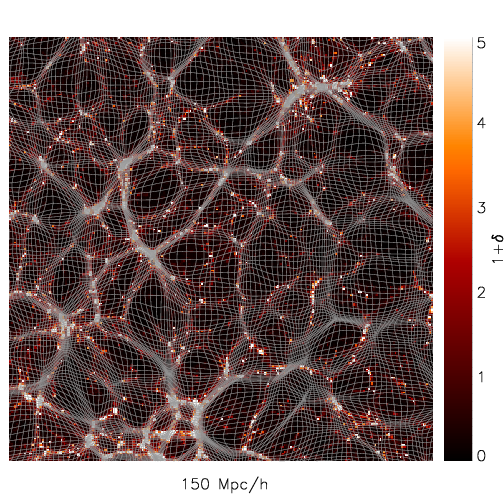
\includegraphics[width=5.5in]{Figures/map0512-0128_i1500_.png}}
\end{picture}
\vspace{-3in}
\titlepage
}

%\section*{Introduction}


\begin{comment}
  \subsection{Outline}

  \frame{
    \frametitle{Outline}
    \tableofcontents
  }
\end{comment}
\section{Reconstruction}
  \frame{
\vspace{-0.5in}
    \frametitle{History}
    \begin{itemize}
      \item in memory: Fred Kwok-Yung Lo
        \item Seo, Eisenstein, etc: displacements
        \item signal loss, noise increase (Ngan et al 2012)
        \item Mass coordinates: Zhu et al 2016
        \item reverse N-body: Tully-Peebles, Goldberg, Wang (ELUCID)
        \item 
     \end{itemize}
  }

\frame{
\vspace{-0.5in}
    \frametitle{1-D}
    \begin{itemize}
        \item McQuinn\&White
        \item unique mass coordinate
        \item closest non-parametric reconstruction (Zhu et al 2016)
     \end{itemize}
  }
\frame{
    \frametitle{3-D: E-mode}
%\vspace{-0.5in}
\hspace{-0.2in}\includegraphics[width=2.3in]{Figures/nonlinear.png}  
\vspace{0.15in}\includegraphics[width=2.21in]{Figures/reconstructed.png}  

(from Yu et al 2016, 1610.7112)
  }

  \frame{
    \frametitle{Low noise limit}
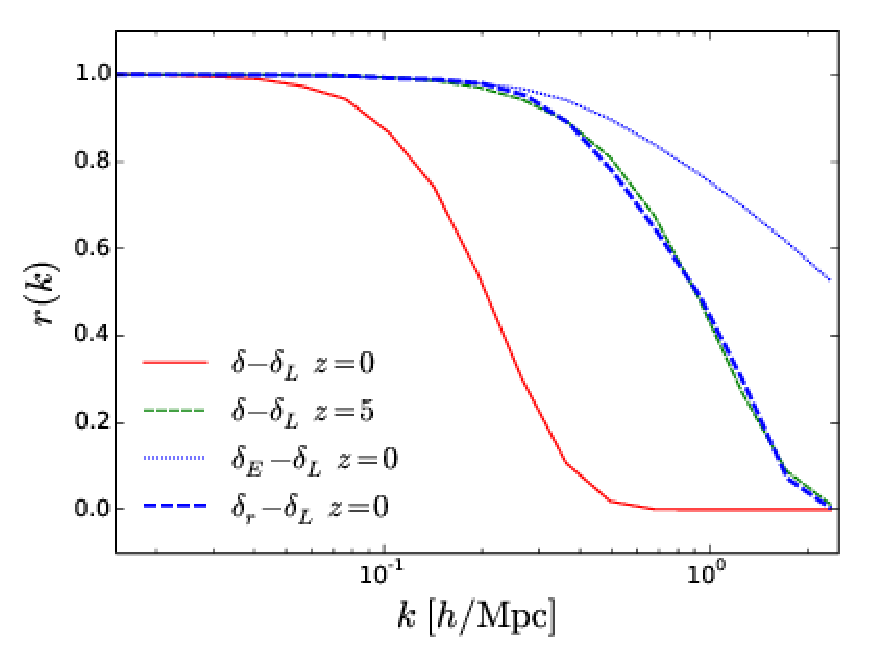
\includegraphics[width=3.4in]{Figures/rk.pdf}

}
  \frame{
    \frametitle{Low noise limit}
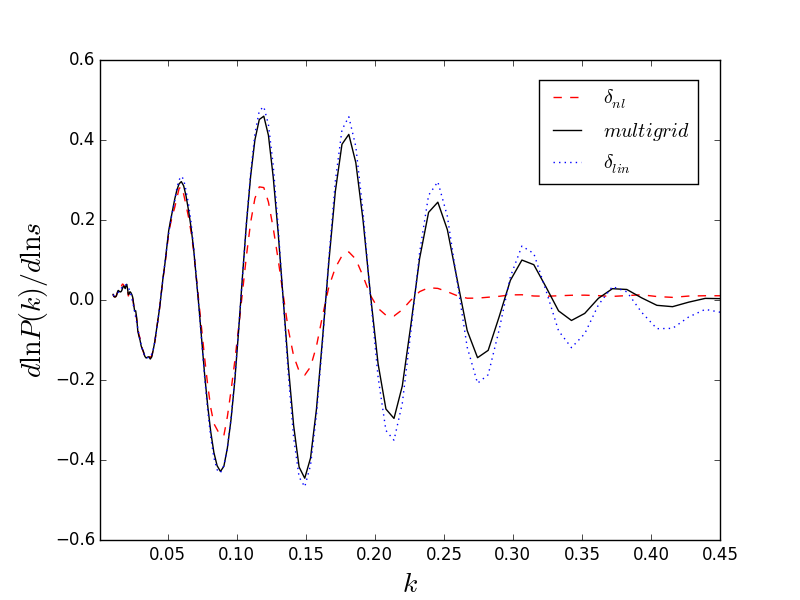
\includegraphics[width=3.4in]{Figures/dlnpk_dlns.png}

}
  \frame{
    \frametitle{Low noise limit}
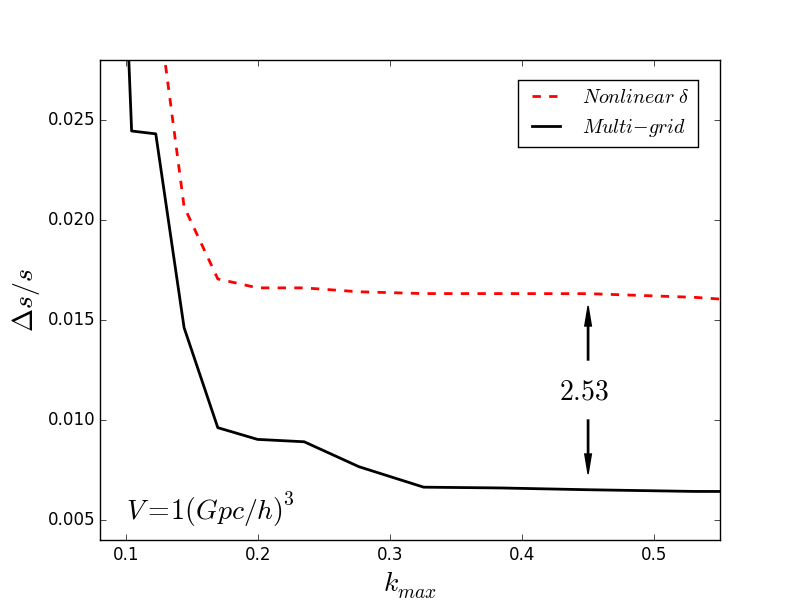
\includegraphics[width=3.4in]{Figures/BAOerr.png}

}

  \frame{
\vspace{-0.5in}
    \frametitle{low z, low noise, 21cm Surveys}
    \begin{itemize}
        \item tunable: Parkes, Tianlai, BINGO
        \item Highjacking: Apertif, GMRT, ASKAP, SKA
        \item 
     \end{itemize}
  }

  \frame{
\vspace{-0.5in}
    \frametitle{Science applications}
    \begin{itemize}
        \item BAO: leverage from low-z where dark energy dominates
        \item neutrino, RSD
        \item 

     \end{itemize}
  }


\frame{
\vspace{-0.5in}
    \frametitle{Conclusions}
    \begin{itemize}
        \item most precise non-parametric reconstruction mechanism to date
        \item well suited for low shot noise low z BAO surveys,
          i.e. intensity mapping
        \item 
     \end{itemize}
  }


\end{document}
